\chapter{Background \& Related Work}
\label{chpt:intro}

Due to its high accuracy, \acrfull{dnn} are widely adopted in image classification cloud services, object detection applications, \acrfull{llm}, etc. Meanwhile, as computational resources grow on edge devices, intelligent robots benefit from deep learning models to obtain a more comprehensive perception of the environment than traditional robots. However, deep learning models are vulnerable to adversarial attacks that can manipulate the model output by adding carefully crafted small perturbations to the model input.

This chapter first introduces how deep learning models are employed in safety-critical applications, such as autonomous driving (one type of mobile robot). Then, we review existing adversarial attacks and discuss unexplored research questions. Lastly, we summarize the structure of the thesis and contributions of each chapter.

% For instance, the Amazon Kiva Robot and Alibaba Quicktron Robot can help warehouse staffs find desired items by moving goods shelves. Each robot can perceive the surrounding environment to avoid collisions with other robots, and receive commands from warehouse staff via cloud servers. On the other hand, autonomous driving research teams from Waymo (formerly the Google self-driving car project), Tesla, etc intend to achieve autonomous navigation without human interference.

\section{Deep Learning in Autonomous Driving}
\label{sec:deep_learning}

% \begin{figure}[H]
% \centering
% \begin{subfigure}[b]{0.485\textwidth}
%     \centering
%     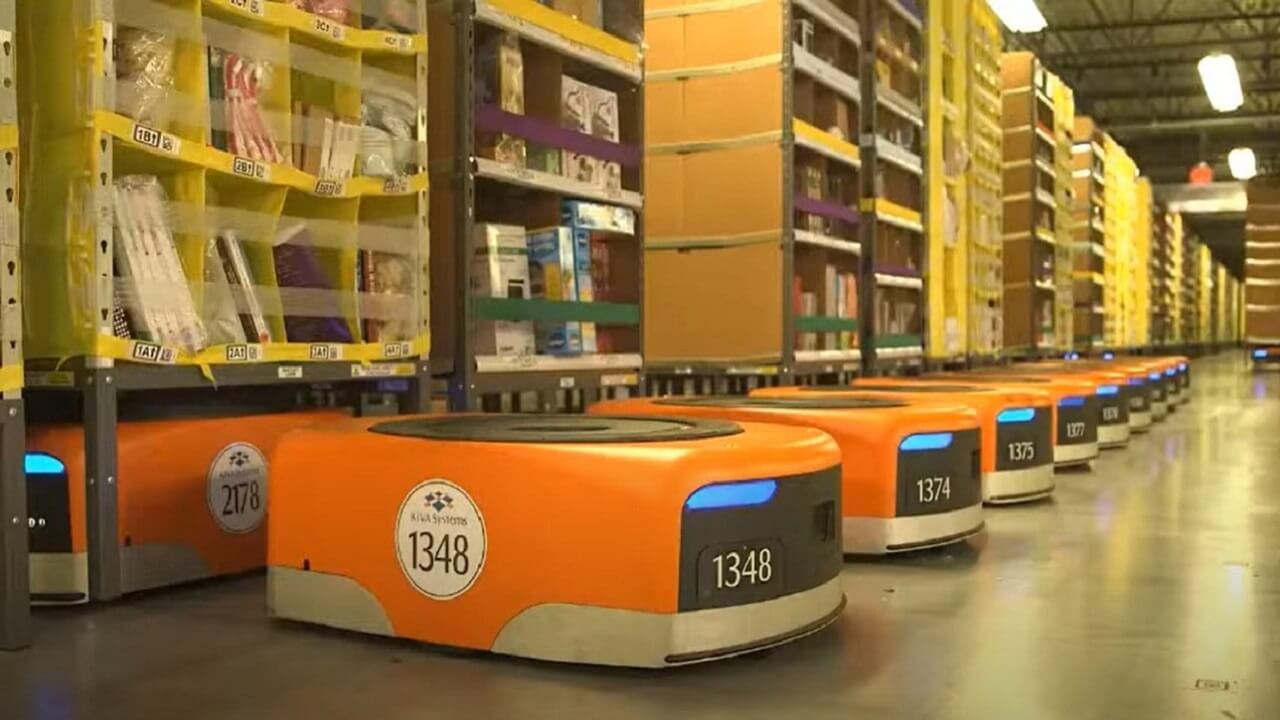
\includegraphics[width=\textwidth]{figures/chapter_intro/amazon_kiva.jpg}
%     \caption{Amazon Kiva Robot}
%     \label{fig:kiva}
% \end{subfigure}
% \hfill
% \begin{subfigure}[b]{0.485\textwidth}
%     \centering
%     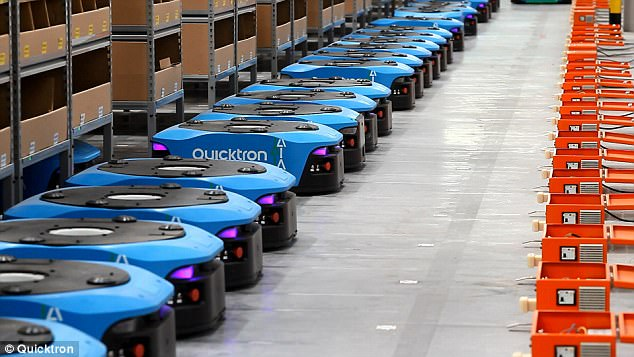
\includegraphics[width=\textwidth]{figures/chapter_intro/alibaba_quicktron.jpg}
%     \caption{Alibaba Quicktron Robot}
%     \label{fig:quicktron}
% \end{subfigure}
% \hfill
% \caption{Robots in warehouse.}
% \label{fig.robot}
% \end{figure}

% \begin{figure}[H]
% \centering
% \begin{subfigure}[b]{0.485\textwidth}
%     \centering
%     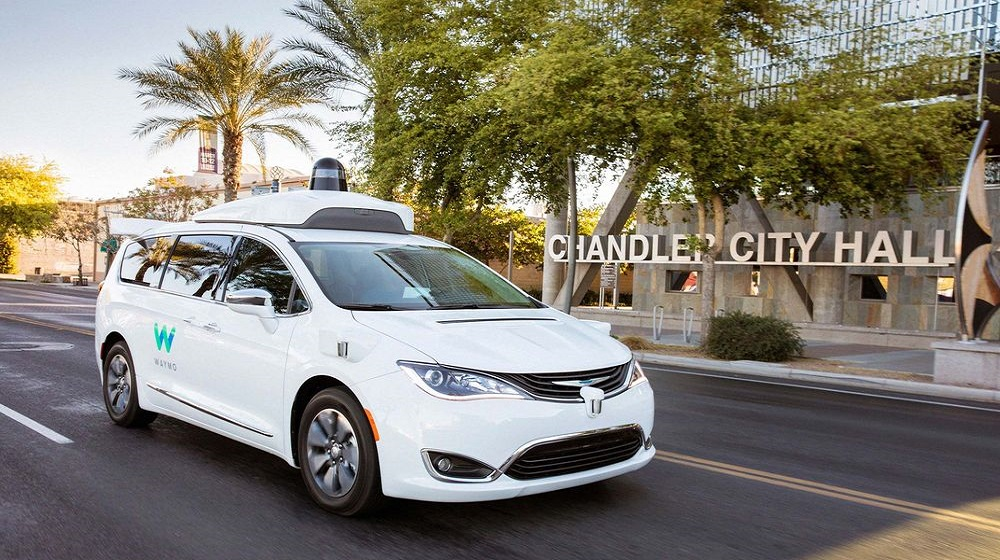
\includegraphics[width=\textwidth]{figures/chapter_intro/waymo.jpg}
%     \caption{Waymo (formerly Google self-driving project)}
%     \label{fig:waymo}
% \end{subfigure}
% \hfill
% \begin{subfigure}[b]{0.485\textwidth}
%     \centering
%     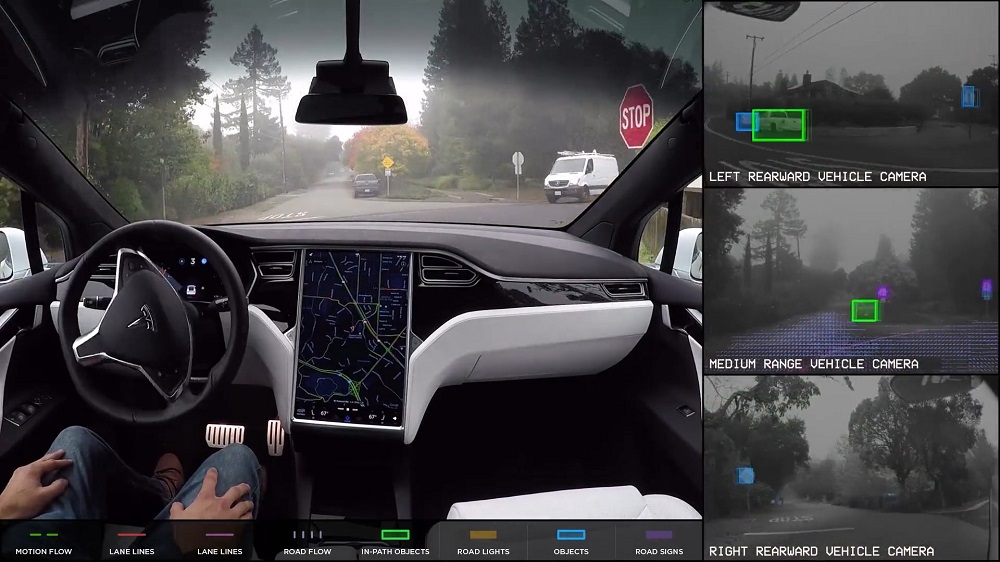
\includegraphics[width=\textwidth]{figures/chapter_intro/tesla_autopilot.jpg}
%     \caption{Tesla Autopilot}
%     \label{fig:tesla}
% \end{subfigure}
% \hfill
% \caption{Autonomous Driving Research}
% \label{fig.autonomous}
% \end{figure}

% As the research in deep neural networks advances, deep convolutional networks become feasible for automated driving tasks. Our research investigates the effect of adversarial attacks against deep learning models.

Autonomous driving stands out as a successful application of deep learning, leveraging deep neural networks to enable self-driving technology. Companies like Waymo (previously the Google self-driving car project) and Tesla are at the forefront of this innovation, aiming to create autonomous vehicles capable of navigating complex environments without human intervention.

% Autonomous Driving is an example of a successful deep learning application that employs deep neural networks. Research teams from Waymo (formerly the Google self-driving car project), Tesla, etc intend to achieve autonomous navigation without human interference.

Following the established divide-and-conquer engineering principle, autonomous driving systems are commonly designed as modular systems that divide the driving task into subtasks: localization, perception, prediction, planning, and control \citep{pendleton2017perception}. 

Through the localization module, the vehicle determines its position in the environment. The perception module enables vehicles to collect information and extract relevant knowledge from the environment. Then, the prediction module predicts future measurements, behavior, trajectory, etc. Lastly, the planning module makes purposeful decisions to achieve the goal, and the control module executes the planned actions. In addition to modular systems, end-to-end driving that maps inputs directly to steering commands has started to rise as an alternative to modular systems.

Unfortunately, both modular systems and end-to-end driving models are vulnerable to adversarial attacks. It is risky to attack real-world autonomous driving systems, while the development of physics engines and realistic renderers makes it feasible to test adversarial attacks in photorealistic simulators.
 
% \subsubsection{Deep Learning}
% \label{sec:deep_robot}

The CARLA simulator is an open-source platform for autonomous driving simulation based on the Unreal Game Engine (see Fig. \ref{fig:carla_intro}). It simulates various sensors such as depth camera, 3D lidar, and radar. In addition, the Carla simulator provides flexible Python APIs to interact with virtual environments and supports \acrfull{ros} integration \citep{Dosovitskiy17}.

\begin{figure}[H]
\centering
\begin{subfigure}[b]{0.49\textwidth}
    \centering
    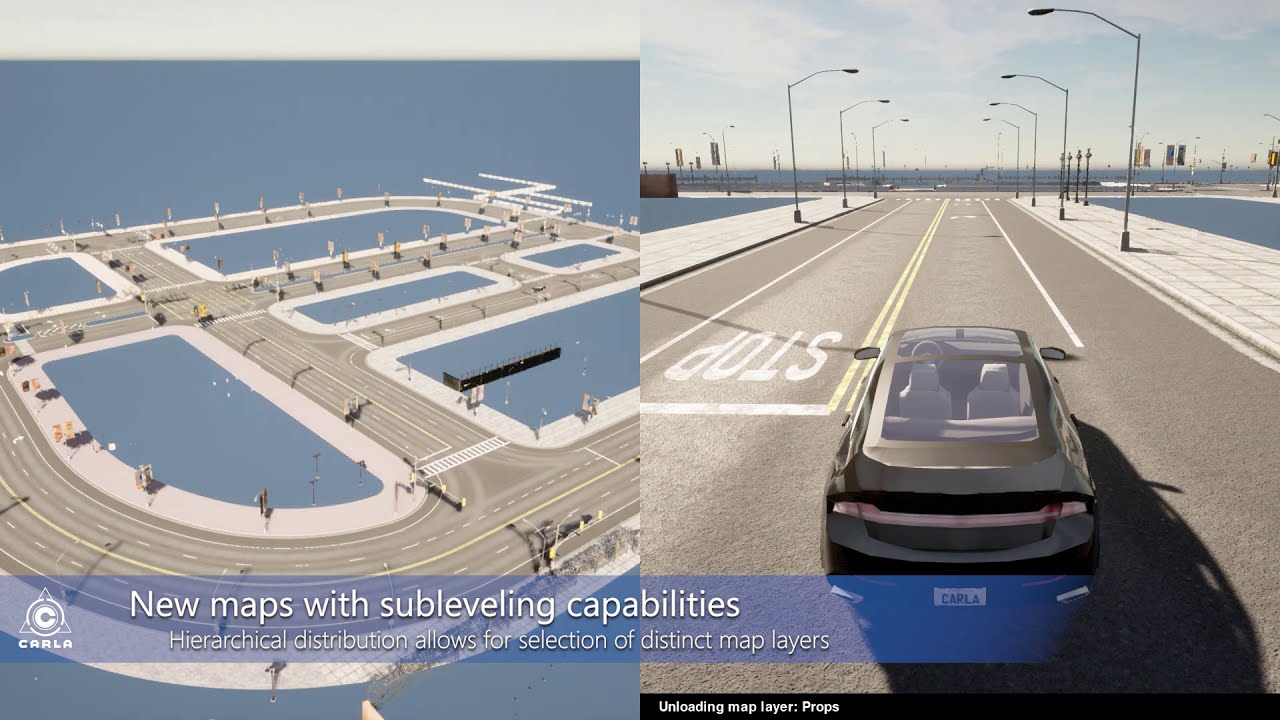
\includegraphics[width=\textwidth]{figures/chapter_intro/carla.jpg}
    \caption{CARLA Simulator \citep{Dosovitskiy17}}
    \label{fig:carla_intro}
\end{subfigure}
\hfill
\begin{subfigure}[b]{0.49\textwidth}
    \centering
    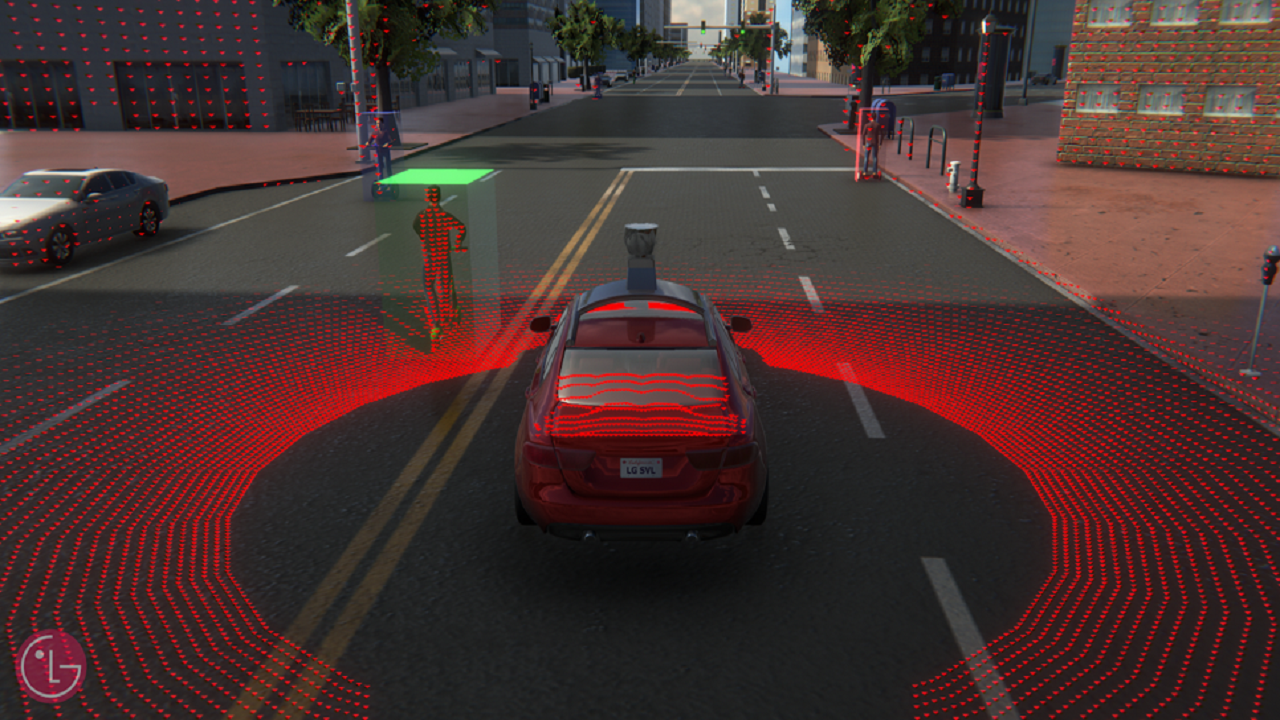
\includegraphics[width=\textwidth]{figures/chapter_intro/lgsvl.png}
    \caption{LGSVL Simulator\citep{rong2020lgsvl}}
    \label{fig:lvsvl}
\end{subfigure}
\hfill
\caption{Autonomous Driving Simulators}
\label{fig.simulator}
\end{figure}

 LGSVL is another platform for autonomous vehicle simulation based on the Unity3D game engine (see Fig.\ref{fig:lvsvl}). It provides integration with the Baidu Apollo platform \citep{rong2020lgsvl}. Both the CARLA simulator and the LGSVL simulator focus on autonomous driving simulation. On the other hand, the Microsoft Airsim simulator provides virtual environments for autonomous driving and drone simulation \citep{airsim2017fsr} (see Fig. \ref{fig.airsim}).

\begin{figure}[H]
\centering
\begin{subfigure}[b]{0.49\textwidth}
    \centering
    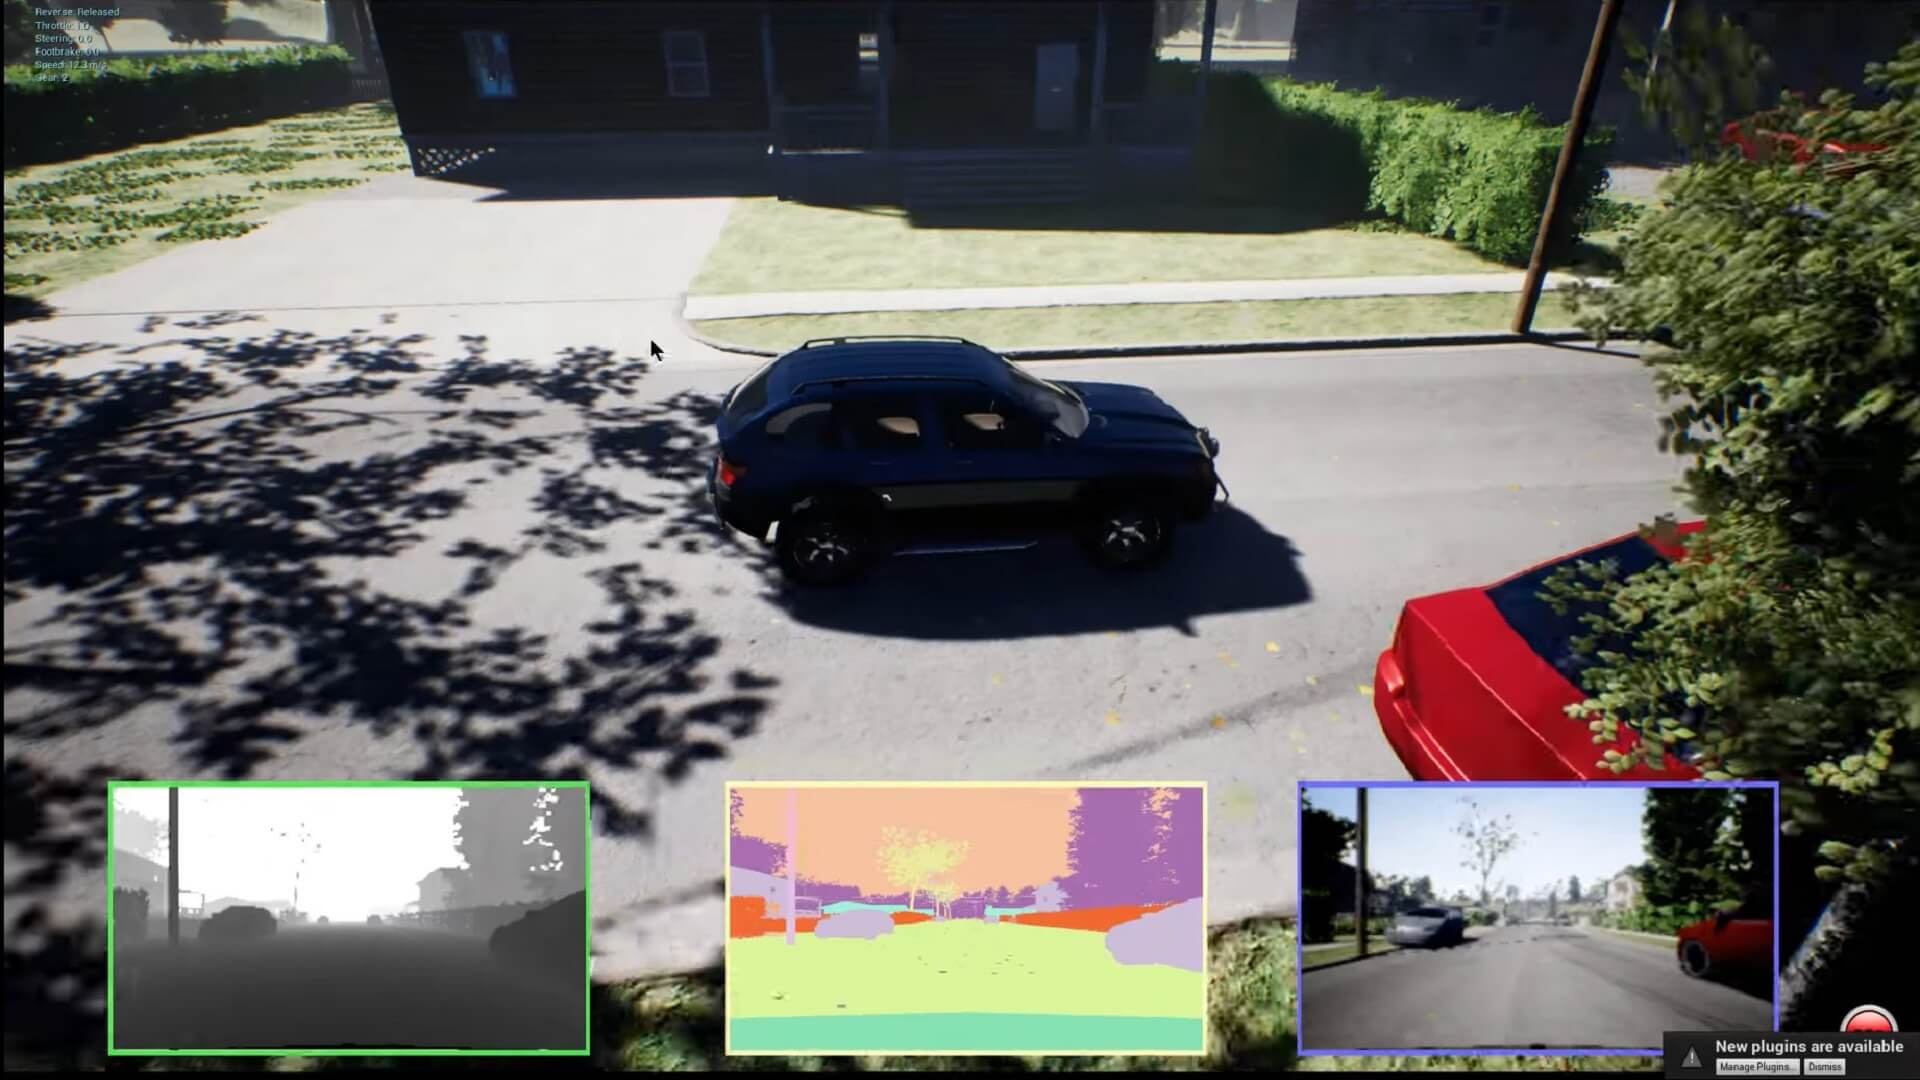
\includegraphics[width=\textwidth]{figures/chapter_intro/airsim_car.jpg}
    \caption{Airsim for Autonomous Vehicles}
    \label{fig:airsim_car}
\end{subfigure}
\hfill
\begin{subfigure}[b]{0.49\textwidth}
    \centering
    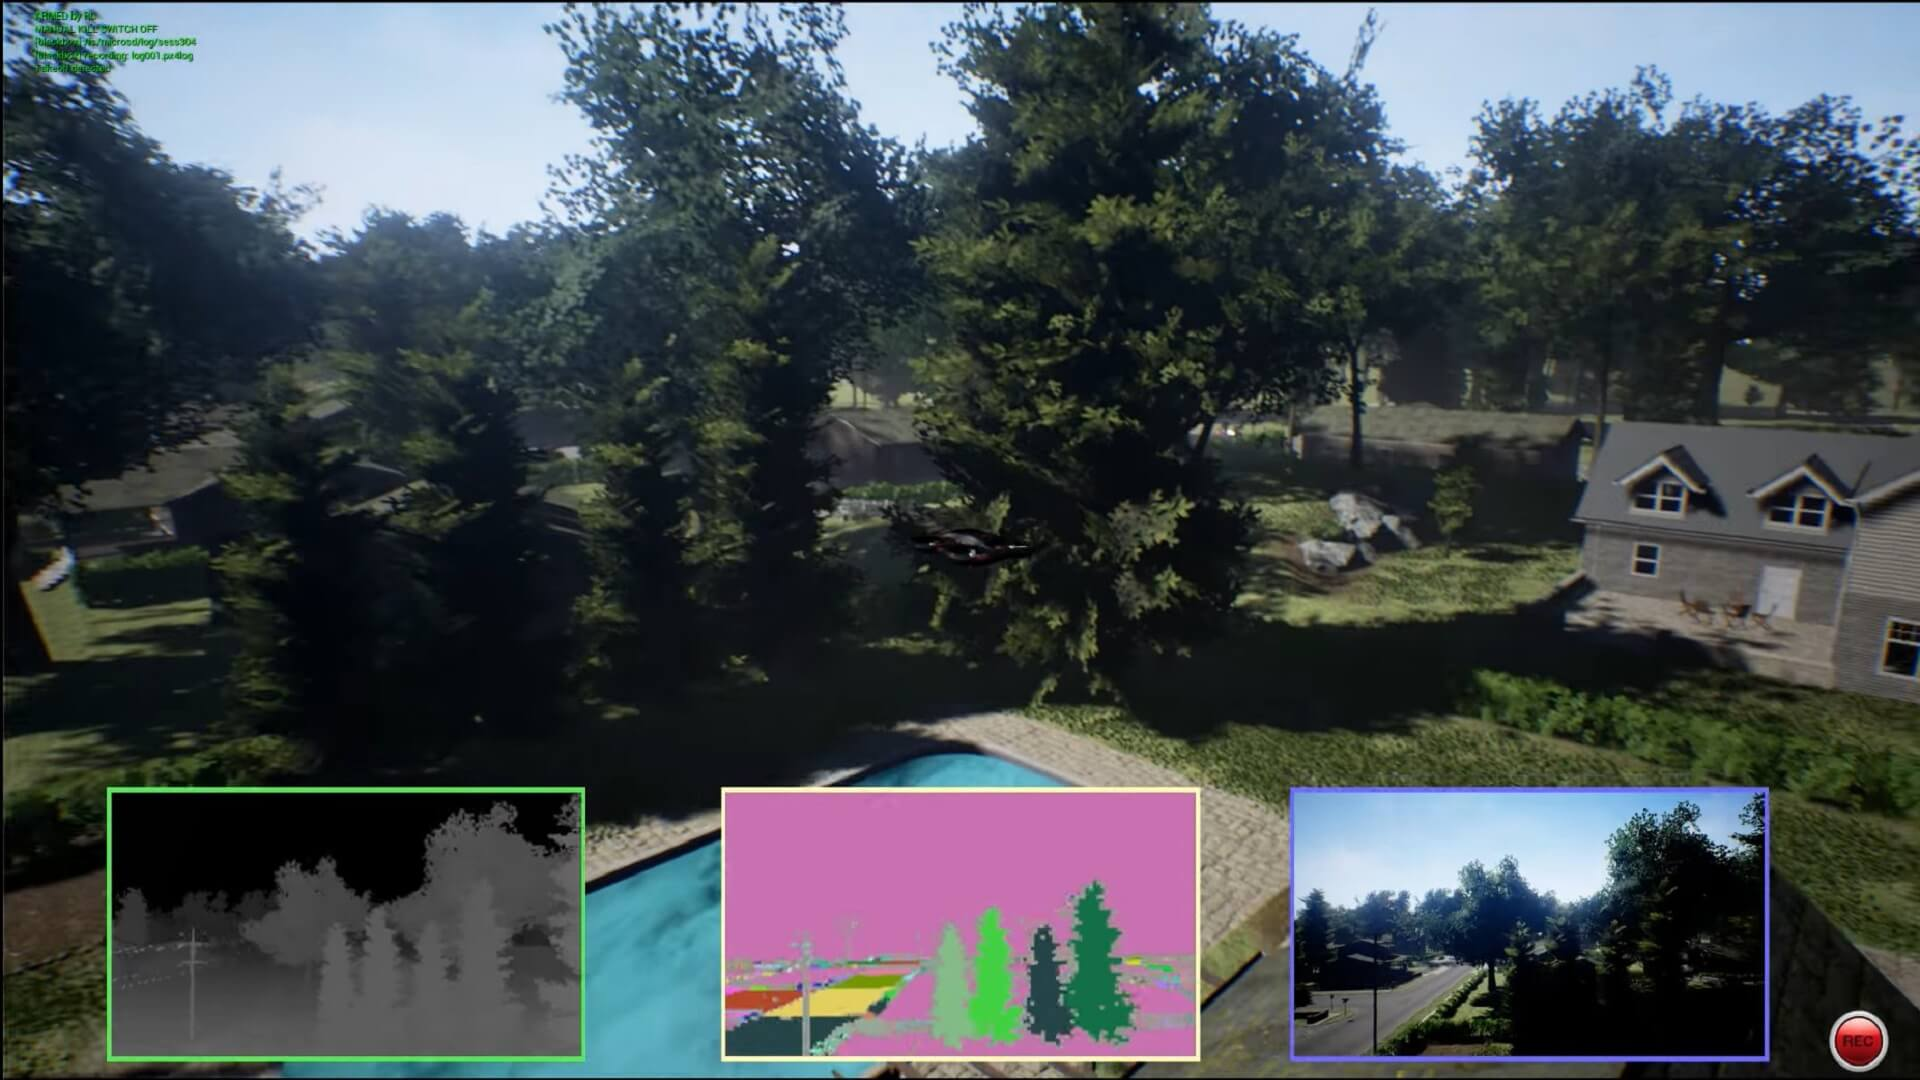
\includegraphics[width=\textwidth]{figures/chapter_intro/airsim_drone.jpg}
    \caption{Airsim for Drones}
    \label{fig:airsim_drone}
\end{subfigure}
\hfill
\caption{Microsoft Airsim Simulator \citep{airsim2017fsr}}
\label{fig.airsim}
\end{figure}


% \section{Deep Learning in Healthcare}
% \label{sec:healthcare}

% Deep learning models are also extensively used in safety-critical healthcare applications. More recently, these models played significant roles in identifying biomarkers and making diagnoses, particularly during the COVID-19 pandemic. 

% As the virus spread rapidly, it became essential to promptly screen a large group of people and isolate infected individuals. Reverse Transcription Polymerase Chain Reaction (RT-PCR) is commonly used to detect viruses from respiratory secretions in acute respiratory infections, which can also be employed to diagnose COVID-19, as confirmed by \citet{corman2020detection}. However,  the demand for the RT-PCR test exceeded hospitals' capacity in many countries. Besides, false negatives could occur if the sample contains insufficient quantities of the virus at the early stage of infection. As a result, diagnostic and predictive models were implemented to assist in fast screening and relieve pressure on healthcare workers.

% Chest CT imaging is a common technique for diagnosing pneumonia and can also assist in COVID-19 confirmation. However, discriminating COVID-19 pneumonia from non-COVID-19 pneumonia poses a challenge to medical practitioners. Matsuyama et al. proposed a wavelet-based CNN system to address this challenge \citep{matsuyama2020deep}. Instead of using the raw image, the neural network takes the wavelet coefficients of the original image as inputs (see Fig. \ref{fig.healthcare} left). Although deep neural networks can achieve high accuracy, they often sacrifice interpretability. To improve interpretability, gradient-weighted class activation mapping is employed to highlight the areas the CNN model focuses on, ensuring that the model's predictions align with medical knowledge.

% Although CT chest imaging can assist in COVID-19 confirmation, the patient throughput is limited because a deep cleaning of the CT examination room is necessary before imaging the next patient \citep{kwee2020chest}. Utilizing biomarkers from routine tests, such as complete blood count (CBC) and inflammatory markers, as inputs to machine learning models could be beneficial. Yan et al. developed a rule-based decision tree model that employs three biomarkers—lactic dehydrogenase (LDH), lymphocyte count, and high-sensitivity C-reactive protein (hs-CRP)—selected by machine learning models to make predictions \citep{Yan2020} (see Fig. \ref{fig.healthcare} right). The model is small and interpretable while still achieving over 90\% accuracy.

% The wavelet-based CT chest imaging system that uses deep neural networks is vulnerable to adversarial attacks. Although the small decision tree model is interpretable, it relies solely on three biomarkers for prediction, limiting its capacity for more complex tasks.

% \clearpage

% \null
% \vfill

% \begin{figure}[H]
% \centering
% 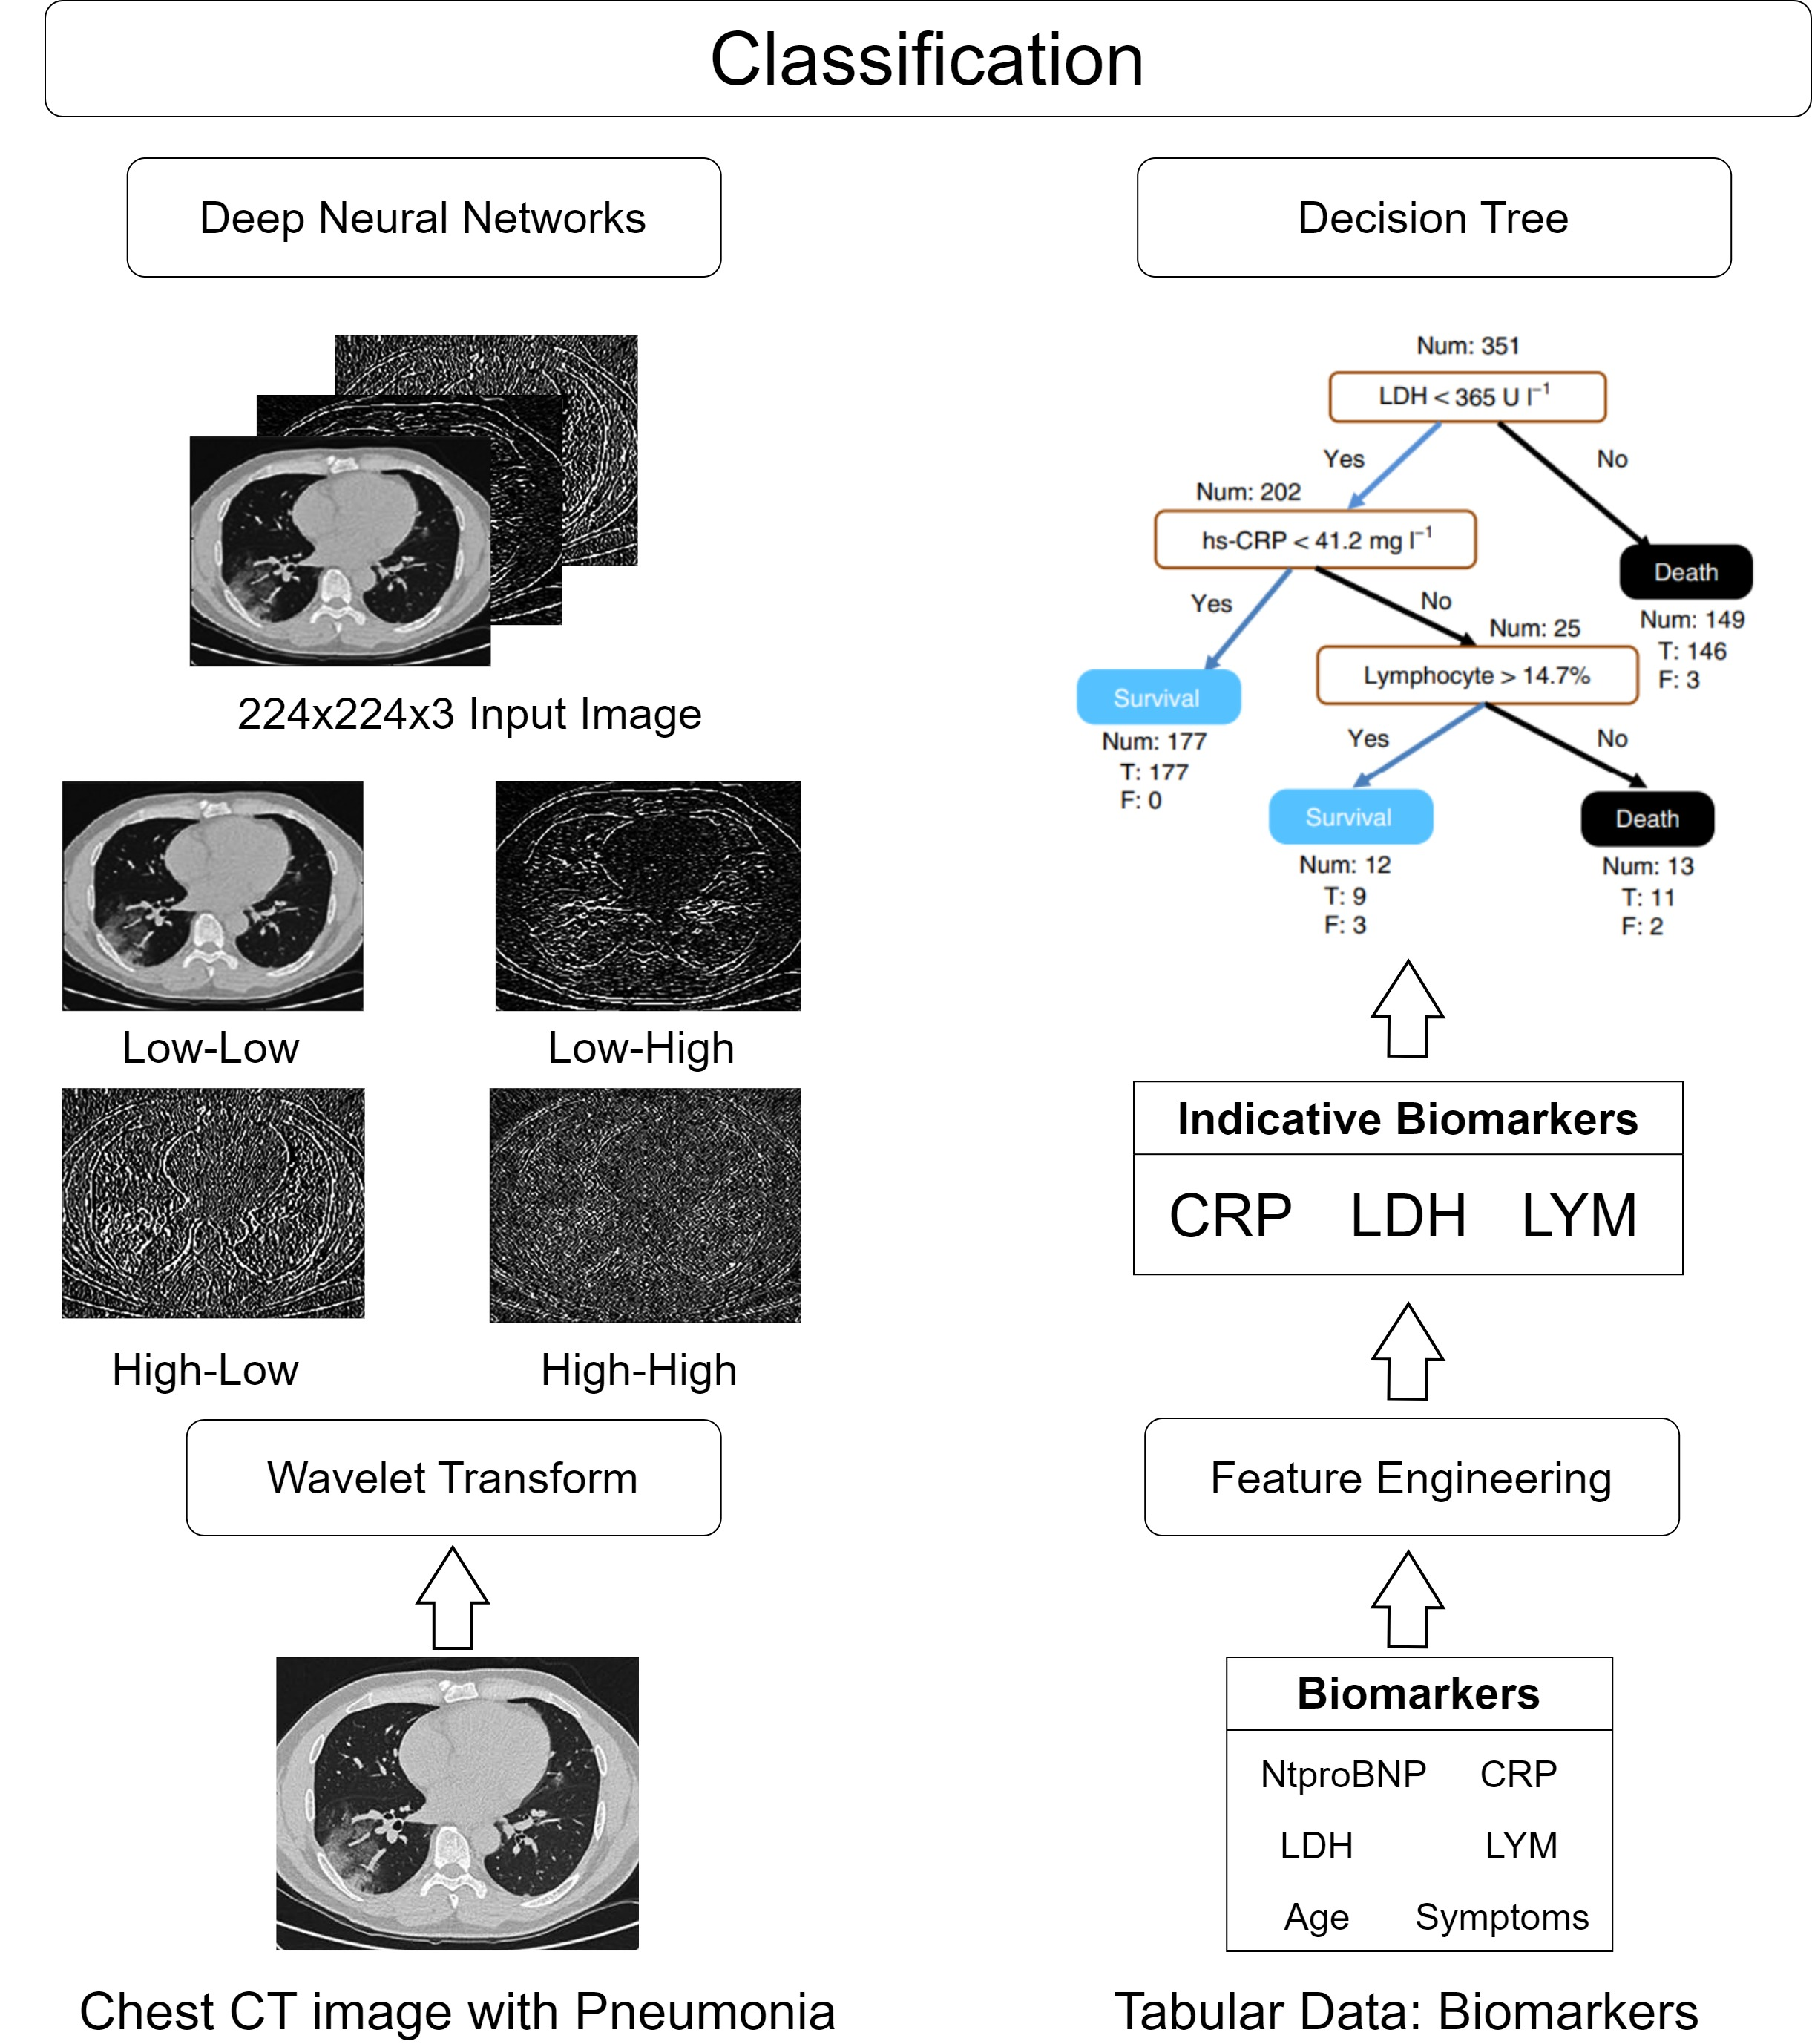
\includegraphics[width=\textwidth]{figures/chapter_intro/healthcare.jpg}
% \caption{Two approaches to COVID-19 severity prediction \citep{matsuyama2020deep, Yan2020}.}
% \label{fig.healthcare}
% \end{figure}

% \vfill

% \clearpage

\section{Review of Adversarial Attacks}
\label{sec:adv_attack}

The existence of adversarial examples was first identified by Biggio et al. \citep{biggio2013evasion} and Szegedy et al. \citep{szegedy2013intriguing}. They fooled a classification model by adding a small perturbation to the input image. Existing adversarial attacks can be categorized into white-box, gray-box, and black-box attacks. 

In white-box attacks, the adversaries have full knowledge of the target model, including the model architecture and parameters. In gray box attacks, adversaries only have limited access to the training set, the model structure, the model parameters, and the model output. In black-box attacks, adversaries can only gather information about the target model by querying \citep{REN2020346}. This thesis focuses on white-box and black-box attacks, since the boundary between gray-box and black-box attacks is rather unclear. For instance, gray-box attacks with no access to predicted probabilities are also known as label-only black-box attacks.

% Depending on the goal of the attack, adversarial attacks can be further categorized into three types, evasion, poisoning, and extraction attacks \citep{art2018}. Evasion attacks cause models to make incorrect predictions by adding perturbations to the input during inference. The poisoning attack injects malicious data into the training set. Lastly, the extraction attack steals or replicates models that are available to query. For autonomous systems, rather than trying to steal models or poison others' training data, we intend to design a system that is resistant to malicious perturbations in the input. Thus our research object coincides with evasion attacks.

\subsection{White-Box Attacks}
\label{sec:whitebox_attack}

White-box attacks rely on gradients to deceive deep learning models. In the training process, samples from the training set are fed forward through the model, and gradients are backpropagated from the training loss to the model parameters using the chain rule. Then, gradients are used to update the model parameters to minimize the training loss. For adversarial attacks, the gradients are backpropagated from the adversarial loss to the input of the model. Using different adversarial loss functions, adversaries achieve different attack objectives. The strategy of updating and applying the perturbation also varies. Next, we use image classification models as target models to formulate white-box attacks (see Fig. \ref{fig.adv_perturb}).

\begin{figure}[H]
\centering
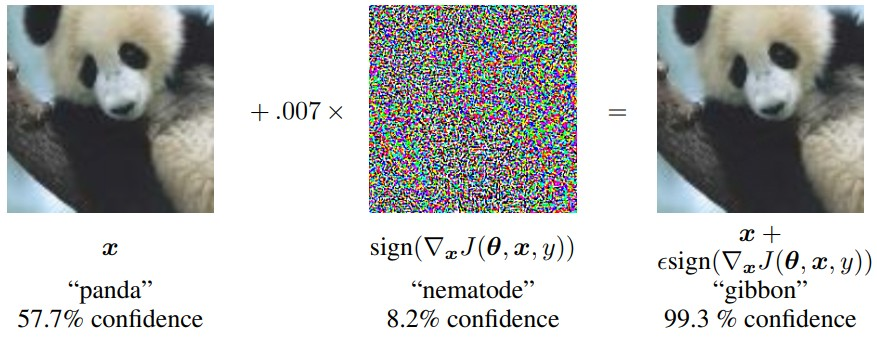
\includegraphics[width=0.95\textwidth]{figures/chapter_intro/fgsm.jpg}
\caption{The \acrfull{fgsm}\citep{GoodfellowSS14} is the first gradient-based white-box attack.}
\label{fig.adv_perturb}
\end{figure}

\subsubsection{Problem Formulation}

Taking image classification models as an example, the deep learning model is denoted as $f(\cdot)$ with input $x$ and prediction $f(x, \theta)$, where $\theta$ are the model weights. The corresponding optimization loss is denoted by $\mathcal{L}(f(x, \theta), y^*)$, where $y^*$ is the ground truth. An adversarial input $x'$ is close to the original input $x$ under a distance metric, while $f(x', \theta) \neq f(x, \theta)$. Formally, an adversarial example is defined as follows:

\begin{equation}
x^{'}: ||x - x^{'}|| < \xi, f(x', \theta) \neq f(x, \theta)
\end{equation}
where $ \xi$ is a predefined distance constraint on the maximum allowed perturbation. The most commonly used distance metric is the $L_p$ distance metric. The distance between $x$ and $x'$ is denoted as $||x-x'||_{p}$, where $||\cdot||_p$ is defined as follows:

\begin{equation}
 ||\textbf{v}||_p = (|v_1|^p + |v_2|^p + \dots + |v_d|^p)^{1/p}
\end{equation}
where $p$ is a real number and $d$ is the dimension of the vector $\textbf{v}$. For instance, the $L_0$ distance corresponds to the number of pixels being modified in the perturbation. The $L_2$ distance measures the standard Euclidean distance between $x$ and $x'$, and the $L_\infty$ distance measures the maximum element-wise difference between $x$ and $x'$.

With full access to model structure and parameters, white-box attacks \textbf{maximize} the loss function $\mathcal{L}(f(x, \theta), y^*)$ by adding noise to \textbf{ model inputs} $x$, while deep learning models are trained by \textbf{minimizing} the loss function $\mathcal{L}(f(x, \theta), y^*)$ by updating \textbf{ model weights} $\theta$.

\subsubsection{Adversarial Perturbation}

The first gradient-based white-box attack is \acrfull{fgsm} \citep{GoodfellowSS14} that generates adversarial inputs using:

\begin{equation}
x' = x + \xi \cdot \text{sign}(\ \bigtriangledown_x \mathcal{L}(f(x, \theta), y^*)\ )    
\end{equation} 
where $\text{sign}(\cdot$) calculates the element-wise sign of a given matrix and $\bigtriangledown_x \mathcal{L}(f(x, \theta), y^*)$ is the gradient of the input $x$ with respect to the loss $\mathcal{L}(f(x, \theta), y^*)$.

The \acrshort{fgsm} generates the adversarial example in one step, while the \acrfull{pgd} \citep{madry2017towards} transforms the \acrshort{fgsm} attack into a \textbf{multi-step attack} that updates the perturbation at each iteration while remaining the overall perturbation $x^{'}$ in a $L_p$ ball using the projection function $\texttt{proj}_{p}(\cdot)$:

\begin{equation}
x'_{t+1} = \text{proj}_{p}(x'_t + \xi \cdot \text{sign}(\ \bigtriangledown_x \mathcal{L}(f(x, \theta), y^*)\ ))
\end{equation}

% \clearpage

\subsubsection{\acrfull{uap}}

The multi-step \acrshort{pgd} attack is further improved by the Deep Fool attack \citep{moosavi2016deepfool} that adds the norm of the gradient difference while iterating over each class $k$ at each step $t$:

\begin{equation}
x'_{t+1} = x'_t + \frac{|f_k(x^{'}_{t}, \theta) - f_{k^{*}}(x^{'}_{t}, \theta)|}{||\omega'_{\hat{k}}||^2_2} \text{sign}(\omega'_{\hat{k}})
\end{equation}
where the $k^*$ is the ground truth class label and $f_k(\cdot)$ is the predicted probability of class $k$. $x_0$ is the original input image without adversarial perturbations. $\omega'_k$ is the gradient difference between the gradient calculated using the original image and the adversarial image:  $\omega'_k = \bigtriangledown_x \mathcal{L}(f(x', \theta), y^*) - \bigtriangledown_x \mathcal{L}(f(x_0, \theta), y^*)$.

\textbf{From image-specific attack to image-agnostic attack:} So far, we have only introduced image-specific attacks that generate adversarial perturbation for each input image. As image-specific attacks become more and more effective while keeping human-unperceivable, another research question arises: can we produce an image-agnostic perturbation that can attack all images in a dataset?

Based on the Deep Fool attack, Moosavi-dezfooli et al. generate \acrshort{uap}s, represented with $\textbf{v}$, by further projecting the overall perturbation to $L_p$ ball of radius $\xi$ and centered at 0 after iterating over each class $k$ \citep{moosavi2017universal}:

\begin{equation}
\text{proj}_p(\textbf{v}, \epsilon)= \arg\ \underset{\textbf{v}_{t+1}}{\min}||\textbf{v}_{t+1} - \textbf{v}_{t}||_2 \quad \text{subject to}\ ||\textbf{v}_{t+1}||_p\leq\xi
\end{equation}

\begin{figure}[H]
\centering
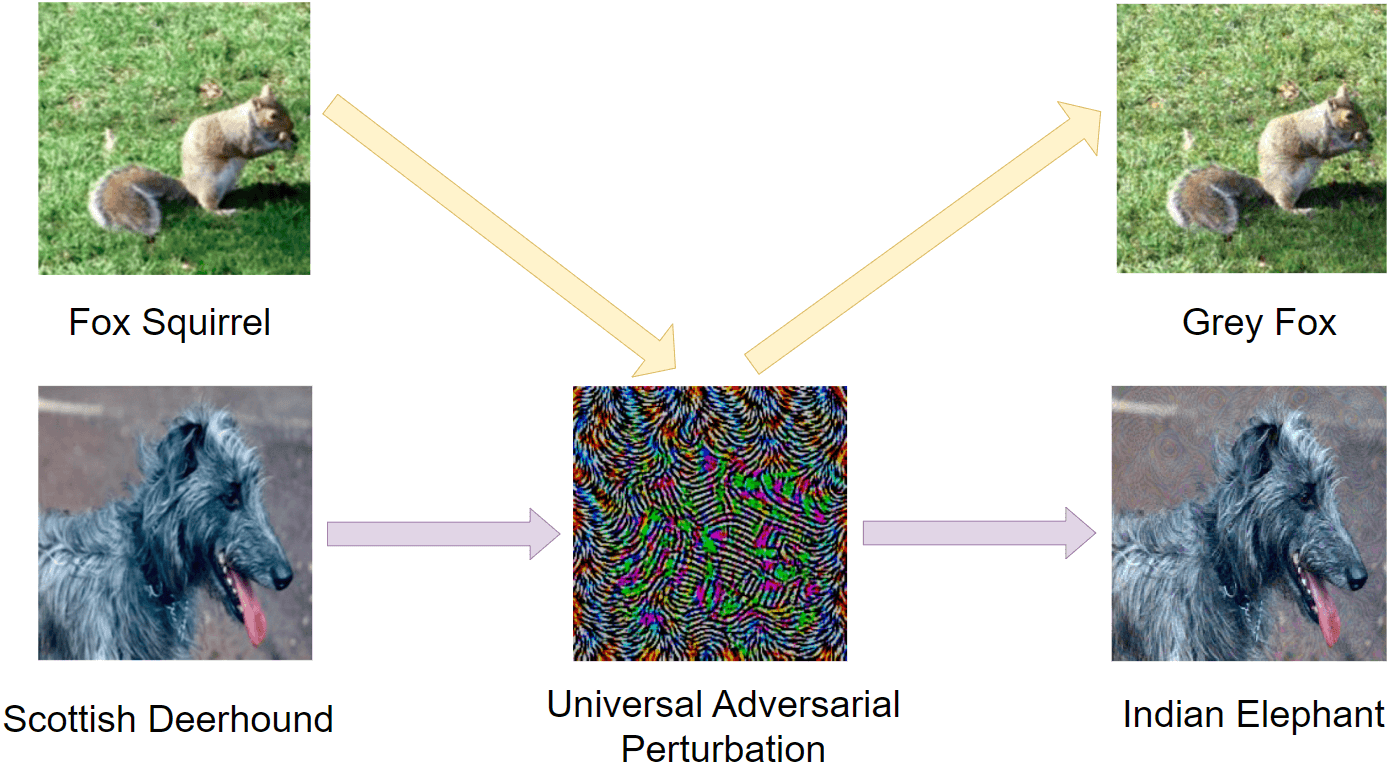
\includegraphics[width=0.9\textwidth]{figures/chapter_intro/uap.png}
\caption{The \acrfull{uap} attacks different images using the same perturbation.}
\label{fig.uap}
\end{figure}

% \clearpage

\subsubsection{Digital Patch}

As illustrated in previous sections, adding a small and intentional drift to the input distribution, also known as adversarial perturbations, can substantially decrease the deep neural network's performance. Digital patches apply adversarial perturbations by directly modifying image pixel values. However, the effectiveness of the adversarial perturbation is limited by the maximum allowed perturbation. What if the adversaries prioritize the attack success rate over imperceptibility, which means that we can remove the constraint of imperceptibility?

In addition to applying a small adversarial perturbation to the entire image, we can also add a human-noticeable patch to a small region of the input image to opt for a more effective (see Fig. \ref{fig:digital_patch}). Besides, the effectiveness of adversarial patches should be position invariant. Digital patches can fool the model without overlapping with target objects \citep{saha2020role}.


\begin{figure}[H]
\centering
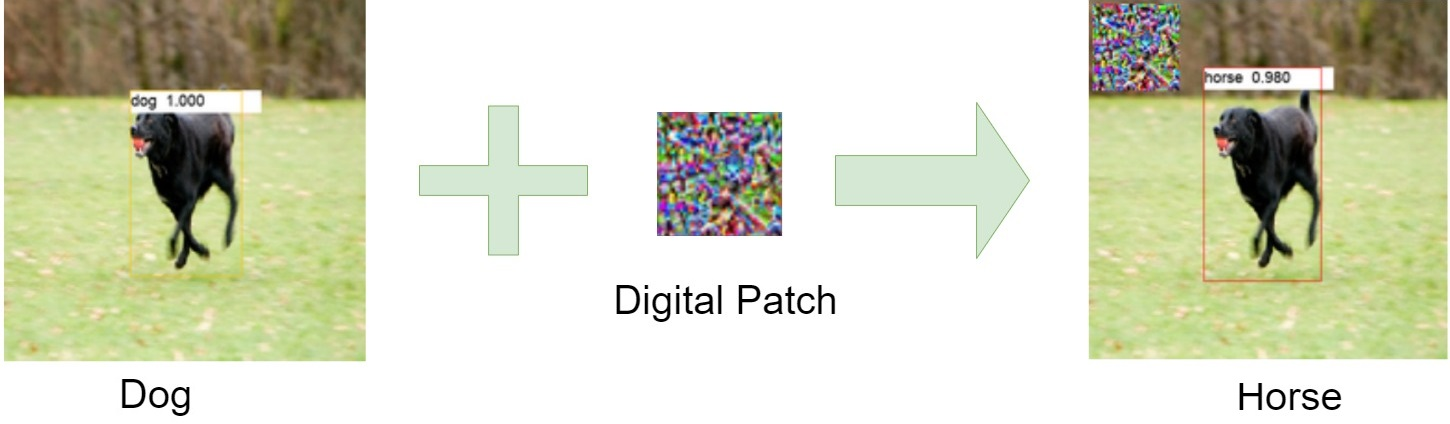
\includegraphics[width=0.95\textwidth]{figures/chapter_intro/digital_patch.jpg}
\caption{The digital patch attacks the image by modifying pixel values.}
\label{fig.digital_patch}
\end{figure}


% A variant of the Expectation over Transformation (EOT) framework \citep{athalye2018synthesizing} is used to obtain the trained patch. In particular, the patch is trained to optimize the objective function:

% $$\hat{p} = \arg \underset{p}{\max}\mathbf{E}_{x \sim X, t \sim T,l \sim L}[logPr(\hat{y}|A(p,x,l,t))]$$

% where $X$ is a training set of images, $T$ is a distribution over transformations of the patch, and $L$ is a distribution over locations in the image \citep{brown2018adversarial}.

% \clearpage

\subsubsection{Physical Patch}

In 2017, Brown et al. brought adversarial examples to the physical world by printing human-noticeable patches on stickers \citep{brown2017patch}, posing threats against real-world applications (see Fig. \ref{fig.physical_patch}). The physical patch is trained using 10,000 images from the training set, applying a random translation, scaling, and rotation to the patch in each image.

Later, research interests gradually shifted from digital attacks to physical attacks. The digital DPatch \citep{liu2018dpatch} was extended to the physical world \citep{lee2019physical} by adding expectation over transformations to find a physical patch:

\begin{equation}
\hat{p} = \arg \underset{p}{\max}\ \mathbf{E}_{x \sim X, t \sim T}\ \mathcal{L}[f(A(x', p, t), \theta), y^*]
\end{equation}
where $A(\cdot)$ is a “patch application function” that transforms the patch
$p$ with the transformation $t$ sampled from a series of transformations $T$.

\begin{figure}[H]
\centering
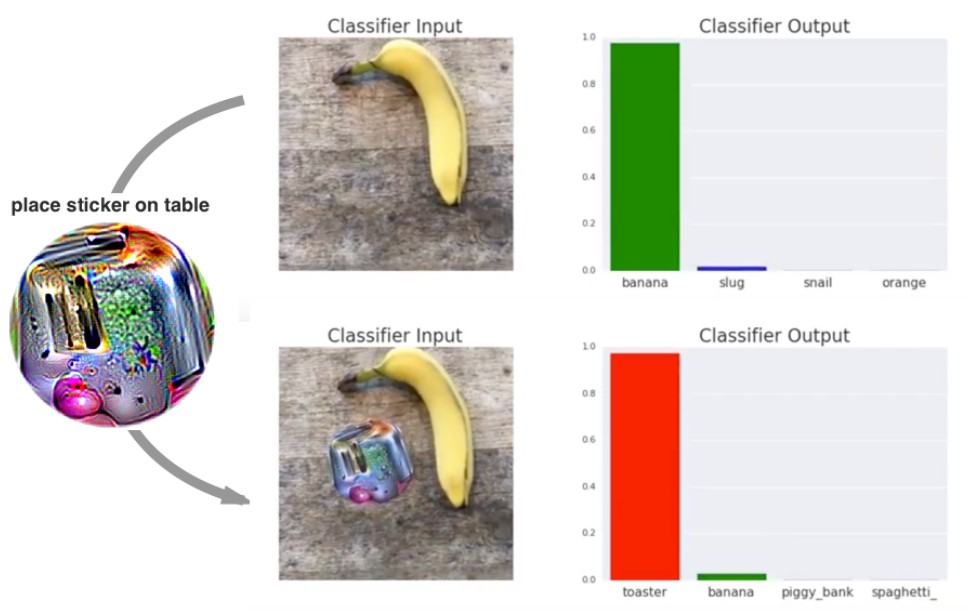
\includegraphics[width=\textwidth]{figures/chapter_intro/adv_patch.png}
\caption{Physical Patch: the adversarial patch is printed and placed on the table \citep{brown2017patch}.}
\label{fig.physical_patch}
\end{figure}

The physical patch can be further improved by adding the \acrfull{nps} as extra constraints to the optimization loss function:

\begin{equation}
\hat{p} = \arg \underset{p}{\max}\mathbf{E}_{x \sim X, t \sim T}\ \mathcal{L}[f(A(x', p, t), \theta), y^*] + SNPS(p, \beta)
\end{equation}
where $\beta$ is the sampling rate and the \acrfull{snps} is used to measure the image printability, or in other words, the error between a printed pixel and its digital counterparts \citep{wang2021daedalus}. However, some research generates asterisk and grid-shaped patches \citep{wu2020dpattack} or small patches \citep{huang2021rpattack} to reduce the number of perturbed pixels, making it infeasible to be printed out on physical objects.

The reason that physical patches are visually perceptible by human eyes is that they must be able to be captured by sensors (e.g. cameras). As a result, physical attacks require a substantial intensity of perturbations. In a survey on physical attacks, Wei et al. categorized adversarial patches into meaningful patches and meaningless patches that do not correspond to real-world objects \citep{wei2023visually}. For example, Chindaudom et al. produce meaningful patches by combining patches with QR Codes \citep{chindaudom2020adversarialqr, chindaudom2022surreptitious}. 

\begin{figure}[H]
\centering
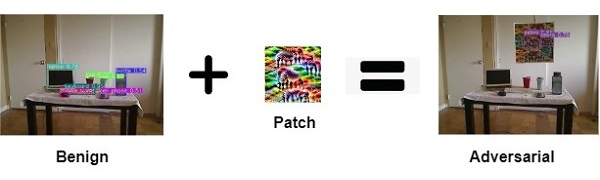
\includegraphics[width=\textwidth]{figures/chapter_intro/physical_patch.png}
\caption{The physical patch can either be attached on the target object or does not overlap with target objects.}
\label{fig.physical_patch_overlap}
\end{figure}

Physical patches pose great threats to autonomous driving vehicles because they are invariant to input images and therefore can inherently achieve real-time attacks \citep{threet2021physical}. For example, previous research generates stop signs that cannot be recognized by object detection models \citep{song2018physical} \citep{chen2019shapeshifter}, and adversarial posters to vanish pedestrians \citep{thys2019fooling, wang2021towards}. Besides, physical patches do not necessarily need to overlap with target objects (see Fig. \ref{fig.physical_patch_overlap}).

Although most patches are static, Hoory et al. generate and display dynamic patches on a monitor attached to a vehicle \citep{hoory2020dynamic}. However, physical patches can only attack object detection models when the camera is close enough \citep{wang2021daedalus, lu2021scale}.

On the other hand, although most physical attacks are visually perceptible by human eyes, some optical attacks can only be captured by sensors (e.g., rolling shutter attacks) but not by human eyes. Li et al. summarized optical adversarial attacks, including attacks that use high-frequency light, a laser, and a projector in \citep{li2022survey}.

% Our research will focus on adversarial patches that are noticeable by human eyes. In \cite{sharma2022adversarial}, Sharma et al. surveyed adversarial patch attacks in vision-based tasks that involve three mainstream models: classification, detection, and re-identification \cite{wei2022physical}, and we will focus on adversarial attacks against object detection models.

% \clearpage

\subsection{Black-Box Attacks}
\label{sec:blackbox_attack}

White-box attacks rely on gradients computed through back-propagation to generate adversarial examples efficiently. However, gradients are not available for real-world deep learning applications because backpropagation is essential only for training, but not for inference. Without access to gradients, white-box attacks become infeasible in the real world. As a result, black-box attacks become promising for attacks against deep learning cloud services.

\subsubsection{Problem Formulation}

Taking black-box attacks against image classification models as an example, the adversary has no access to the model structure and model weights and can only generate adversarial perturbations via sending queries to the model (see Fig. \ref{fig.decision}).
 
Given an input image $x$, the objective of the adversary is to fool a black-box image classifier $f(x)$ by adding a small perturbation $\delta$ to the original image and generate an adversarial image $x^{'} = x + \delta$, such that $f(x^{'}) \neq f(x)$. Unlike white-box attacks, note that adversaries have no access to model parameters $\theta$ under black-box settings. Typically, the perturbation $\delta$ is bounded in the $l_2$ or $l_{\infty}$ norm by some user-defined constant.

Decision-based black-box attacks only require access to the predicted class (hard label), while score-based attacks also require the probability of each predicted class (soft label).  Next, we introduce the two most popular strategies for black-box attacks: gradient estimation and local search.

\begin{figure}[H]
\centering
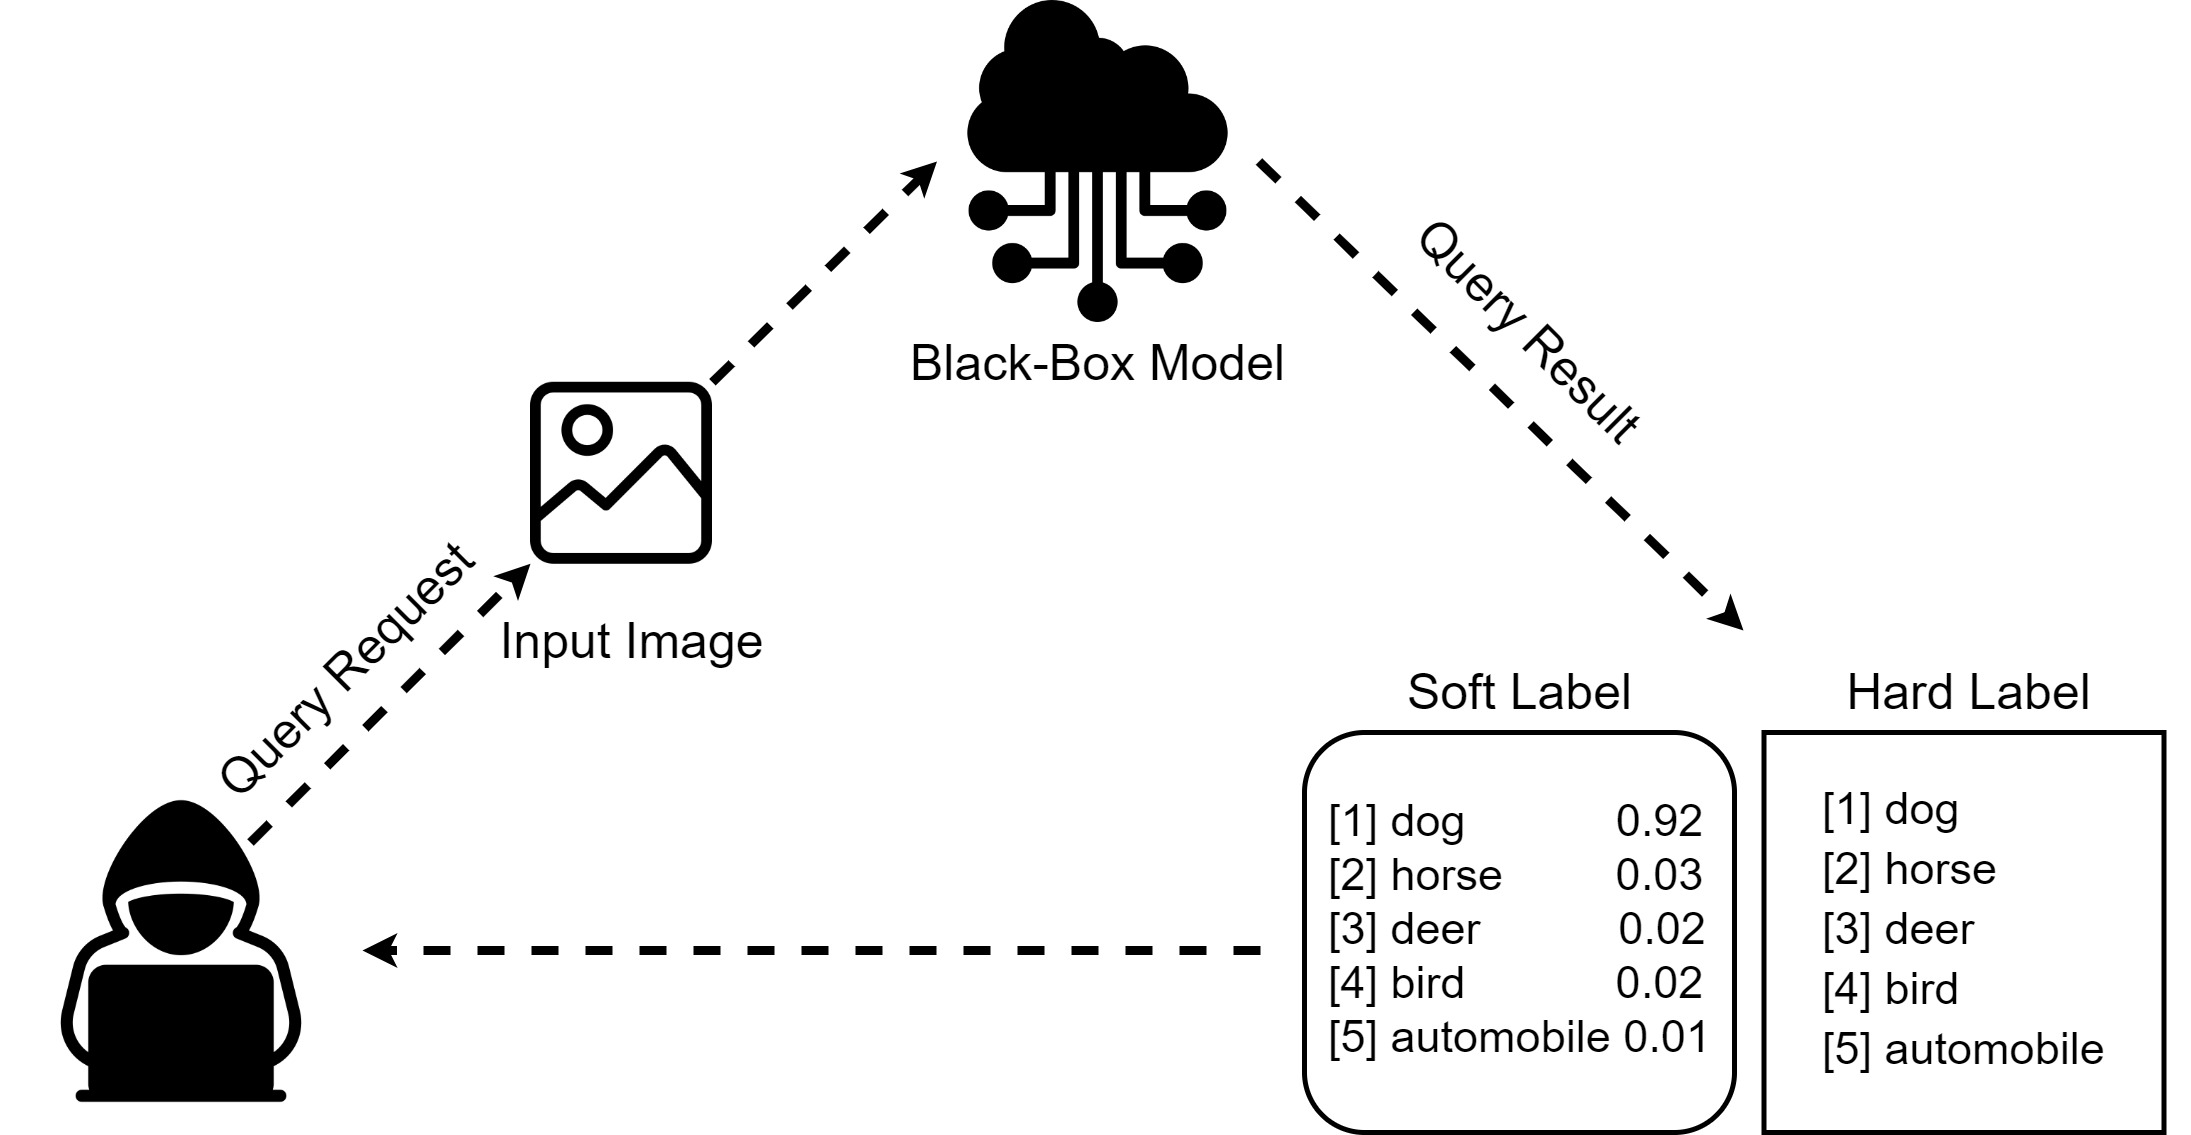
\includegraphics[width=\textwidth]{figures/chapter_intro/black-box.jpg}
\caption{The Black-Box Adversarial Attack.}
\label{fig.decision}
\end{figure}

% \clearpage

\subsubsection{Gradient Estimation}

Intuitively, if we can estimate gradients by slightly changing the model input and observing the model output, we can exploit existing white-box attacks to generate adversarial examples. For example, the \acrfull{zoo} Attack amends the C\&W white-box attacks to the black-box setting by approximating gradients using a finite difference method \citep{chen2017zoo}. The original C\&W attack generates adversarial examples $x'$ by solving the optimization problem:

\begin{equation}
    \text{minimize}\ ||x'-x||^2_2 + c \cdot F(x', t)
\end{equation}
where $F(x', t)$ is the regularization function and $c>0$ is a regularization parameter. The target class is represented with $t$.

To solve the above optimization problem, we need access to the gradients of the regularization function with respect to the input $\bigtriangledown_{x^{'}} F(x^{'}, t)$, which is not available in black-box settings. Thus, the \acrshort{zoo} attack estimates the gradient using a finite difference method rather than backpropagation:

% \begin{equation}
%     \frac{\partial^2 F(x)}{\partial x^2} \approx \frac{F(x+he_i) - 2F(x) + F(x-he_i)}{h^2}
% \end{equation}

\begin{equation}
    \frac{\partial F(x)}{\partial x} \approx \frac{F(x+he_i) - F(x-he_i)}{2h}
\end{equation}
where $h$ is a small step size (e.g. $h = 0.0001$), and $e_i$ is a standard basis vector with only the i-th component being 1.

Query efficiency is a crucial evaluation metric for black-box attacks, and the following research tries to improve the sample efficiency of gradient estimation using gradient priors and natural gradient estimation.

% \begin{equation}
% f(x,t) = \max \{ {\underset{i \neq t}{\max}\ log[F(x)]_i - log[F(x)]_t, -\kappa } \}
% \end{equation}

% The ZOO Attack relies on the output of confidence scores to estimate the gradient, while decision-based attacks can generate adversarial inputs using even less information.

\subsubsection{Local Search}

On the other hand, local search is another popular black-box attack method. The FGSM attack either adds or deducts a small value to each pixel, indicating that adversarial perturbations are combinations of orthogonal vectors. As a result, local search methods use existing local search methods, such as heuristic search, to search for combinations of orthogonal vectors to decide which pixels to attack.

Intuitively, we can add or deduct a small value to one pixel at a time and choose the operation that decreases the probability of the correct label. The attack is known as \acrfull{simba} \cite{guo2019simple}, a baseline method. However, even for a 32x32 input image, the \acrshort{simba} method takes more than 2000 queries, which is inefficient. To reduce the search space, later research finds combinations of vertical and horizontal lines and square patches rather than individual pixels.

% \clearpage

In addition to gradient estimation and local search, another approach to producing adversarial examples is to use a surrogate model. Surrogate-based black-box attacks generate adversarial perturbations by transferring from a surrogate model, but their attack success rates are lower than gradient-estimation and search-based methods.

Although existing black-box attacks achieve remarkable attack success rates, we notice some common mistakes in prior research that obtain unfair advantages by applying the perturbation before image encoding and preprocessing, thereby overestimating the effectiveness of the attack (see Chapter \ref{chpt:classification}).

\section{Research Questions}
\label{sec:research_question}

Despite rapid progress in generating adversarial examples, many important questions arise for practical adversarial attacks.

\vspace{0.5cm}

\textbf{1) Is it possible to achieve real-time online adversarial attacks?}

Much of the current research on adversarial attacks focuses on offline attacks that utilize both input images $x$ and the corresponding ground truths $y^*$ to maximize adversarial loss $\mathcal{L}(f(x, \theta), y^*)$. However, the human-labeled ground truth $y^*$ is unavailable for real-time online attacks. For example, to attack an object detection model deployed on an autonomous driving vehicle, it is impossible to have humans mark the bounding boxes in real time. Can we generate adversarial perturbations without access to the ground truth?

\vspace{0.5cm}

\textbf{2) Is it possible to inject the perturbations without access to the operating system?}

Access to the operating system is essential in order to inject adversarial perturbations into input images. However, the operating system (Unix / Linux) in which the deep learning model is deployed is highly secure as cyber security research advances. Although the operating system is highly secure, the sensors that collect the data are exposed directly to the environment to collect the data. Can we exploit the sensor to bypass the operating system?

\vspace{0.5cm}

\textbf{3) Can traditional methods mediate the impact of adversarial attacks?}

Although deep neural networks are vulnerable to adversarial attacks, traditional algorithms such as the Kalman Filter and the Hungarian algorithm are not. In real-world robotic applications, deep learning models are deployed in combination with traditional algorithms that do not use deep neural networks. Are adversarial attacks still effective under these settings?

% \vspace{0.25cm}
\clearpage

\textbf{4) Have black-box attacks become a practical threat against commercial Cloud APIs?}
\label{question_4}

IoT devices with limited memory and computational power depend on cloud APIs for tasks such as image classification. Existing black-box attacks report success rates of more than 95\% using fewer than 1,000 queries. This raises the question: Have these attacks become a significant threat to commercial cloud APIs such as Imagga and Google Cloud Vision?

% \clearpage

\section{Thesis Overview \& Contributions}

To answer the research questions listed in Section \ref{sec:research_question}, the remaining of the thesis is organized as follows:

\vspace{0.5cm}

% This thesis presents adversarial attacks against mobile robot perception models, such as image classification, object detection, and object tracking. 

% \begin{itemize}[label={}]

\noindent \textbf{Chapter \ref{chpt:driving}} answers \textbf{research question 1)} by introducing two real-time online white-box attack against the NVIDIA end-to-end driving model, including image-specific and image-agnostic attacks. Both attacks do not require access to the ground truth. We test the attacks in simulation and on real Turtlebots and demonstrate that it is possible to achieve real-time online attacks (\textbf{Published in IEEE Intelligent Vehicle Symposium}). 

\vspace{0.5cm}

\noindent \textbf{Chapter \ref{chpt:detection}} further presents three real-time online white-box attacks against object detection models: the one-targeted attack, multi-targeted attack, and multi-untargeted attack. By combining the imperceptibility of adversarial filters with the localizability of adversarial patches, our method, adversarial overlay, can generate adversarial perturbations of arbitrary shapes at given locations. (\textbf{Published in IEEE Intelligent Vehicle Symposium}). 

To answer \textbf{research question 2)}, we propose a Human-in-the-Middle hardware attack that injects the perturbation into the communication channel between the camera and the detection system, thus bypassing the operating system (\textbf{Published in IEEE Transactions on Artificial Intelligence}). 

\vspace{0.5cm}

\noindent \textbf{Chapter \ref{chpt:tracking}} explores whether traditional algorithms like the Kalman Filter and Hungarian Algorithm, commonly used in object tracking systems, can mitigate adversarial attacks. We evaluated four \acrshort{tbd} frameworks—SORT, Deep SORT, Strong SORT, and OC SORT—combined with YOLOv3, YOLOv4, and YOLOX object detectors on both the KITTI and CARLA datasets. Our findings reveal that the adversarial attack introduced in Chapter \ref{chpt:detection} still compromises tracking models even with the help of traditional methods, addressing \textbf{research question 3}).

\vspace{0.5cm}

\noindent \textbf{Chapter \ref{chpt:classification}} unveils several common mistakes in existing black-box attacks and proposes distributed black-box attacks to accelerate attacks against image classification cloud services and shed light on \textbf{research question4)}. 

Previous research overestimated the effectiveness of black-box attacks by applying the perturbation before image resizing and preprocessing, which is not accessible to end users for commercial image classification cloud APIs. In addition to minimizing the number of queries, black-box attacks can be further optimized by leveraging the load-balancing mechanism commonly used in cloud APIs (\textbf{Under Review for Publication}).

\vspace{0.5cm}

\noindent \textbf{Chapter \ref{chpt:conclusion}} concludes the thesis and envisions future research directions to understand and safely embrace deep learning models. 
